% !TeX spellcheck = fr_FR
% --- --- --- --- --- --- --- --- --- --- --- --- --- --- --- --- %

\documentclass[a4paper,12pt]{report}  % args : article, report, book 
\usepackage[utf8]{inputenc}  % encodage UTF-8 
\usepackage[french]{babel}  % choix de langue, important pour maketitle et tableofcontents
\usepackage{geometry}  % géométrie de la page 
\usepackage{hyperref}  % liens internes et externes 
\usepackage{graphicx}  % images 
\usepackage{longtable}  % tableaux 
\usepackage{fontspec}  % polices d'écriture du système 
\usepackage{tabularx}  % pour des tableaux larges 
\usepackage{lipsum}  % pour du texte 
%\usepackage{titlepic}  % pour avoir une image dans \maketitle
\usepackage{titling}  % pour utiliser \theauthor, \thedate, \thetitle 
\usepackage{datetime}  % pour que la date de \thedate soit en français 
\usepackage{float}  % paramètre 'H' dans figure pour éviter un problème avec les images 
\usepackage{amsmath} % \text dans les équations
\usepackage{listings}

% --- --- --- --- --- --- --- --- --- --- --- --- --- --- --- --- %

\geometry{margin = 2 cm}  % marge de 2 cm (possible d'utiliser "in" aussi)

\setlength{\parindent}{0pt}  % alinéas 
\setlength{\parskip}{.5em}

% hyperref 
\hypersetup{  
	colorlinks=true,
	linkcolor=black,
	urlcolor=blue,
	citecolor=red
}

% fontspec
%\setmainfont{Bricolage Grotesque}
%\setmonofont[size=6pt]{Comic Code Ligatures} 

\lstdefinestyle{mystyle}{language=Python}
\lstset{style=mystyle}



% --- --- --- --- --- --- --- --- --- --- --- --- --- --- --- --- %

\title{Cahier des charges fonctionnel}
\author{
	Alice LIN \\
	Thisalini RAVINTHIRAN \\
	Lilian SAFAR \\
	Djivan VARTANIAN \\
	Benjamin ZHANG \\
	Louise ZHENG \\
}
\date{\today}
%\titlepic{
\includegraphics[width=0.5\textwidth]{../Design/FichiersPoster/Logo_ESIEE.pdf}}

\begin{document}

%	\maketitle

\begin{titlepage}
\centering
\vspace*{9cm} 
{\LARGE \bfseries \thetitle \par}
\vspace{1cm} 
\large \theauthor \par
\vspace{0.5cm} 
\large \thedate \par
\vspace{4cm} 

\includegraphics[width=0.5\textwidth]{../Design/FichiersPoster/PDF/Logo_ESIEE.pdf} 
\vfill 
\end{titlepage}

%	\pagebreak

% --- --- --- --- %

%\section*{Auteurs}
%
%\begin{itemize}
%\item Alice LIN
%\item Thisalini RAVINTHIRAN
%\item Lilian SAFAR
%\item Djivan VARTANIAN
%\item Benjamin ZHANG
%\item Louise ZHENG
%\end{itemize}

% --- --- --- --- %

\tableofcontents

\pagebreak
% --- --- --- --- %

% VENANT DU GOOGLE DOC : COLLER À PARTIR D'ICI
% https://docs.google.com/document/d/1HbEzYS0UaP-KckqQrKnavtIfuLFMVqc9utsnXRt5M9c/ 

\section{Introduction}
% Contexte du projet, problématique, objectifs du robot.

Notre projet vise à développer un robot autonome capable de livrer de la
nourriture ou des boissons de la cafétéria aux personnes se trouvant à
l'ESIEE. Le robot peut se déplacer de manière fluide, mais uniquement le
long du hall.

Une plateforme web sera mise en place permettant aux étudiants et au
personnel de l'ESIEE exclusivement de passer commande en indiquant la
salle dans laquelle ils se trouvent. Via cette même plateforme, ils
pourront également suivre leur livraison en temps réel.

Ce besoin a été identifié lors d'emplois du temps
chargés, par les longues files d'attente ou juste par la
difficulté de certains étudiants à se déplacer.

Ce projet a pour but de clôturer la fin de la première année de notre
cycle ingénieur à l'ESIEE Paris. Il permet de mettre en
application l'ensemble des connaissances acquises lors
de notre formation et d'apprendre davantage sur
d'autres logiciels informatiques et électroniques.

\textbf{Problématique :} Comment concevoir un robot permettant
de livrer de la nourriture aux étudiants depuis la cafétéria ?


\section{Architecture du système}
% Revue des technologies existantes pour la livraison autonome.

\begin{figure}[H]
	\centering
	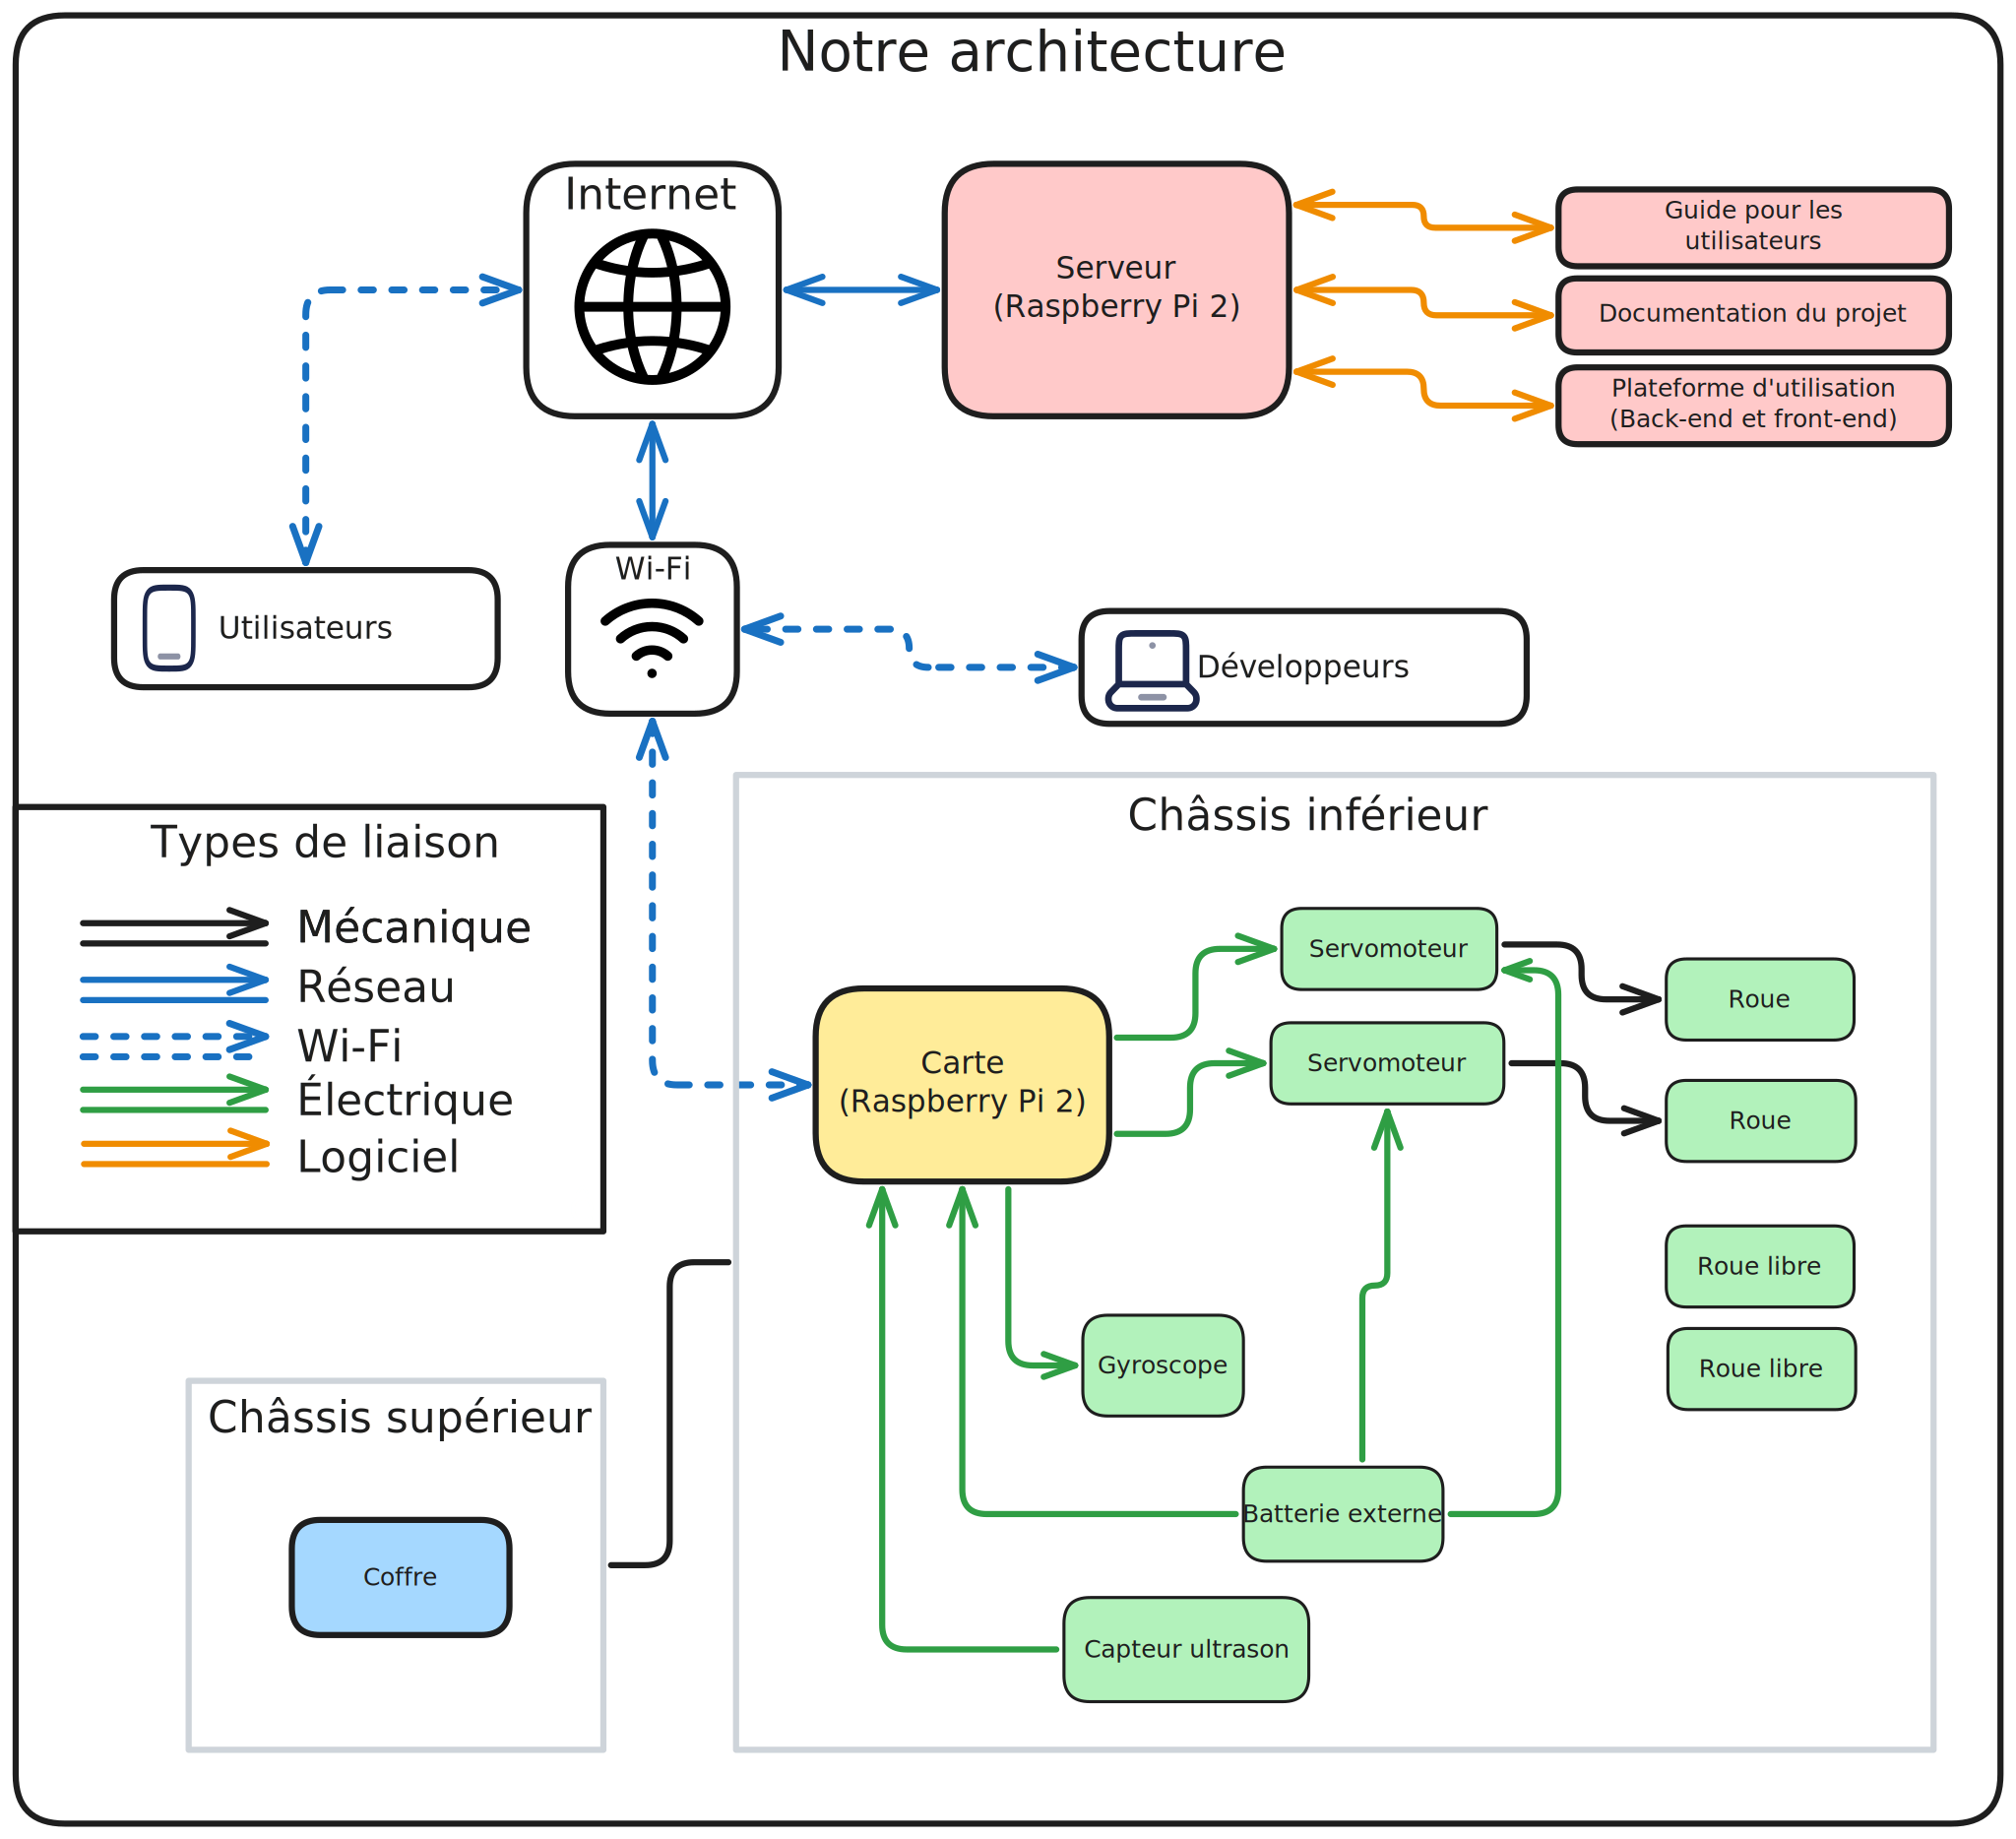
\includegraphics[width=0.6\textwidth]{./attachments/arch/2025-06-21-1200_Architecture.pdf}
	\caption{Schéma de l'architecture. }
\end{figure}

\begin{figure}[H]
	\centering
	\includegraphics[width=0.6\textwidth]{./attachments/sketch.jpg}
	\caption{Schéma du prototype. }
	\label{fig:schema_proto}
\end{figure}

Liste des composants utilisés : 

\begin{itemize}
	%\begin{enumerate}
	\item
	\textbf{Raspberry Pi 4 Model B :} permet de contrôler tous les
	composants.
	
	\item
	\textbf{Module de détection US HC-SR0 :} capteur ultrason qui détecte
	les obstacles.
	
	\item
	\textbf{Servomoteur FB5311M-360 à rotation continue + feedback :}
	permet de faire tourner les roues du robot et l\textquotesingle option
	feedback permet la localisation du robot.
	
	\item
	\textbf{Paire de roulettes pivotantes à platine 
		de diamètre 40 mm (Réf 82629519) :} permet le déplacement du robot.
	
	\item
	\textbf{Paire de roues 136 mm DGR136 :} permet de déplacer le robot à
	l\textquotesingle aide des servomoteurs.
	
	\item
	\textbf{INIU Batterie Externe, 22.5 W 10000 mAh :} permet
	d\textquotesingle alimenter la Raspberry Pi 4 et les servomoteurs
	
	\item
	\textbf{Résistance 2.2 kOhm et 3.3 kOhm :} permet l'utilisation du
	capteur ultrason avec la Raspberry Pi 4.
	
	\item
	\textbf{Breadboard/PCB :} permet de relier tous les composants entre
	eux.
	
	\item
	\textbf{Module capteur LSM9DSO :} composé d'un gyroscope,
	accéléromètre, magnétomètre.
\end{itemize}
%\end{enumerate}



\section{Cahier des Charges Fonctionnel}

\subsection{Description des Fonctionnalités}
% Description des fonctionnalités requises (navigation, évitement d'obstacles, etc.)

{\fontsize{10pt}{12pt}\selectfont 
	\begin{longtable}{|l|l|p{4cm}|p{4cm}|p{4cm}|}
		\hline
		\textbf{Type} & \textbf{N°} & \textbf{Fonctions} 
		& \textbf{Critère de performance} & \textbf{Niveau attendu} \\
		\hline
		\endhead
		
		\hline
		\endfoot
		
		\hline
		Mécanique & F1 & Transporter de la nourriture & Capacité de charge & 3 kg de nourriture  \\
		
		\hline
		Cinématique & F2 & Se déplacer à une vitesse constante réglable & Plage de vitesse réglable & Entre \ldots{} à \ldots{}  \\
		
		\hline
		Électrique & F3 & Avoir une autonomie minimale & Durée de fonctionnement continu sans recharge & Minimum 1 h  \\
		
		\hline
		Logiciel & F4 & Navigation autonome & Itinéraire sans rechargement & \\
		
		\hline
		Mécanique & F5 & Se déplacer de manière stable & Tenue de cap en ligne droite & Pas de déviation significative pendant le trajet (à préciser) \\
		
		\hline
		Informatique & F6 & Circuler en sécurité dans l'établissement & Capacité à contourner des obstacles & Doit éviter humains, murs et objets  \\
		
		\hline
		Informatique & F7 & Détecter les obstacles & Type de détection & Détection fiable pour éviter les collisions \\
		
		\hline
		Mécanique & F8 & Sécuriser la nourriture dans le coffre & Coffre verrouillé mécaniquement & S'ouvre seulement par l'intervention humaine (bouton poussoir, écran)  \\
		
		\hline
		Mécanique & F9 & Assurer la stabilité dans le coffre & Compartimentage adapté & 3 zones : boissons, sandwichs, vide. Le nombre à fixer \\
		
		\hline
		Informatique & F10 & Avoir un site web intuitif pour contrôle utilisateur & Interface simple et claire & Navigation intuitive, accès rapide aux commandes \\
		
		\hline
		Informatique & F11 & Commander le robot via interface web & Contrôle à distance & Envoi d'ordres depuis le site (start/stop) \\
		
		\hline
		Informatique & F12 & Avoir un retour d'information depuis le robot & Données visibles en temps réel & Position, statut, livraison en cours ou terminée, batterie \\
		
	\end{longtable}
}

\subsection{Contraintes Techniques}
% Contraintes techniques (dimensions, poids, autonomie, etc.)

{\fontsize{10pt}{12pt}\selectfont 
	\begin{longtable}{|l|l|p{4cm}|p{4cm}|p{4cm}|}
		\hline
		\textbf{Type} & \textbf{N°} & \textbf{Fonctions} 
		& \textbf{Critères de performance} & \textbf{Niveau attendu} \\
		\hline
		\endhead
		
		\hline
		\endfoot
		
		\hline
		Électrique & T1 & Avoir une batterie adaptée pour l'autonomie &
		Autonomie énergétique & ≥ 1 heure d'alimentation continue \\
		
		\hline
		Cinématique & T2 & Avoir des moteurs adaptés à la charge totale &
		Vitesse fluide & à définir \\
		
		\hline
		Mécanique & T3 & Avoir des roues pouvant supporter la charge & Capacité
		de roulement sous charge & Doivent supporter ≥ charge totale à définir \\
		
		\hline
		Mécanique & T4 & Avoir un coffre assez grand & Volume utile de stockage
		& H = 25 cm, Lg = 40 cm, l = 45 cm \\
		
		\hline
		Logiciel & T5 & Avoir un capteur performant & Portée de détection avant
		& Capteur d'ultrasons : portée de 2 cm à 4 m  \\
		
		\hline
		Mécanique & T6 & Avoir un châssis solide & Résistance mécanique &
		Doivent supporter ≥ \ldots{} kg sans déformation \\
		
		\hline
		Électronique & T7 & Avoir une carte microcontrôleur adaptée & Capacité
		de pilotage & Capacité de pilotage \\
		
		\hline
		Électronique & T8 & Avoir une carte de contrôle double moteur DC &
		Nombre de canaux / compatibilité & Alimenter les moteurs et relier à la
		carte microcontrôleur. \\
		
	\end{longtable}
}



\section{Partie théorique}
On veut dimensionner le moteur, dimensionner la batterie, et rendre le système stable. 

\subsection{Cinématique} 
\subsubsection{Modélisation} 

On cherche la relation entre la vitesse de rotation des roues et la vitesse du robot et sa vitesse de rotation par rapport au sol. 

%![](attachments/schéma_modélisation.jpg)

$S$ est le châssis 
$R_0$ est le référentiel terrestre 
$S_i$ est la roue n°i (il y en a quatre) 
$F_i$ est la fusée n°i (il y en a deux) 

$A_i$ est un point qui représente le point de contact entre la roue n°$i$ et le sol 
$R$ est le rayon de la roue 
$\omega$ est la vitesse de rotation 

$\vec{x},\vec{y},\vec{z} \in S$ 
$\vec{x_0},\vec{y_0},\vec{z_0} \in S_0$ 
$\vec{x_1},\vec{y_1},\vec{z_1} \in F_1$ 
$\vec{x_2},\vec{y_2},\vec{z_2} \in F_2$ 
$S_1$ et $S_2$ sont respectivement confondues avec $F_1$ et $F_2$ 
$S_4$ et $S_3$ sont confondues avec $S$ 

Condition de roulement sans glissement : 
\begin{equation}
	\vec{V}(A_4, S/R_0) = R\omega_{S_4/S} \cdot \vec{x} \tag{1}
\end{equation}
\begin{equation}
	\vec{V}(A_3, S/R_0)=R\omega_{S_3/S} \cdot \vec{x} \tag{2}
\end{equation}

Rotation d'une roue par rapport à $R_0$, obtenu par composition des vitesses de rotation. 
\begin{equation}
	\vec{\Omega}(S_3/R_0) = \omega_{S_3/S} \cdot \vec{y} + \omega_{S/R_0} \cdot \vec{z} \tag{3}
\end{equation}
\begin{equation}
	\vec{\Omega}(S_4/R_0) = \omega_{S_4/S} \cdot \vec{y} + \omega_{S/R_0} \cdot \vec{z} \tag{4}
\end{equation}

%### Étape 1 
Relation entre vitesse de rotation des roues et la vitesse du châssis. 
\begin{equation}
	R\omega_{S_4/S} \cdot \vec{x} + R\omega_{S_3/S} \cdot \vec{x}
	=
	\vec{V}(A_4, S/R_0) + \vec{V}(A_3, S/R_0) 
	\tag{1)+(2}
\end{equation}

Changement de point en $C$. 
$$ = 
\vec{V}(C,S/R_0) 
+ \overrightarrow{A_{4}C} \wedge \vec{\Omega}(S/R_0) 
+ \vec{V}(C,S/R_0) 
+ \overrightarrow{A_{3}C} \wedge \vec{\Omega}(S/R_0) 
$$
$$
= 2\vec{V}(C,S/R_0) + (-\frac{L}{2} + \frac{L}{2}) \cdot \vec{y} \wedge \omega_{S/R_0} \cdot \vec{y}
$$
Donc selon $x$, on a : 
$$
\boxed{
	\vec{V}(C,S/R_0) = \frac{R}{2}\bigg( \omega_{S_4/S} + \omega_{S_3/S} \bigg)
}
$$
%### Étape 2 
Relation entre vitesse de rotation des roues et la **vitesse de rotation** du châssis. 
\begin{equation}
	R\omega_{S_4/S} \cdot \vec{x} - R\omega_{S_3/S} \cdot \vec{x}
	=
	\vec{V}(A_4, S/R_0) - \vec{V}(A_3, S/R_0) 
	\tag{1)–(2}
\end{equation}

Changement de point en $I$, point sur l'axe de rotation du châssis par rapport au sol : $(I,\vec{z})$. 
$$= 
\vec{V}(I, S/R_0) + \overrightarrow{A_4 I} \wedge \vec{\Omega}(S/R_0) 
- \bigg(\vec{V}(I, S/R_0) + \overrightarrow{A_3 I} \wedge \vec{\Omega}(S/R_0) \bigg)
$$
$I$ centre de l'axe de rotation donc $\vec{V}(I, S/R_0) = \vec0$
On a alors : 
$$
= \overrightarrow{A_4 I} \wedge \vec{\Omega}(S/R_0) 
- \bigg( \overrightarrow{A_3 I} \wedge \vec{\Omega}(S/R_0) \bigg)$$
On décompose avec la relation de Chasles : 
$$
= 
\bigg(\overrightarrow{A_4 I_4}+\overrightarrow{I_4 I} \bigg)
\wedge \vec{\Omega}(S/R_0) 
- 
\Bigg( 
\bigg(
\overrightarrow{A_3 I_3} 
+ \overrightarrow{I_3 I_4} 
+ \overrightarrow{I_4 I}
\bigg) 
\wedge \vec{\Omega}(S/R_0) 
\Bigg)
$$

$$
= 
\bigg( -R\vec{z}+\overrightarrow{I_4 I} \bigg)
\wedge {\omega}_{S/R_0} \cdot \vec{z} 
- 
\Bigg( 
\bigg( 
-R\vec{z} + L\vec{y} +\overrightarrow{I_4I}
\bigg) 
\wedge {\omega}_{S/R_0} \cdot \vec{z}  
\Bigg)
$$

$$
= 
- 
\Bigg( 
\bigg( 
L\vec{y} 
\bigg) 
\wedge {\omega}_{S/R_0} \cdot \vec{z}  
\Bigg)
$$

$$
= 
- 
\Bigg( 
\bigg( 
L
\bigg) 
{\omega}_{S/R_0}
\cdot \vec{x}
\Bigg)
$$

Donc : 
$$
R\omega_{S_4/S} \cdot \vec{x} - R\omega_{S_3/S} \cdot \vec{x}
=
-L {\omega}_{S/R_0} \cdot \vec{x}
$$

Selon $\vec{x}$ : 
$$
R\omega_{S_4/S} - R\omega_{S_3/S} 
=
-L {\omega}_{S/R_0} 
$$

Donc : 
$$
\boxed{
	\omega_{S_3/S} - \omega_{S_4/S} 
	=
	\frac{L}{R} {\omega}_{S/R_0}
}
$$

Fin de la cinématique. 

%## Dynamique 
%### Modélisation 
Torseur d'action mécanique avec $i \in \{1,2,3,4\}$ : 
$$
F(\text{route} \to S_i) = 
\begin{Bmatrix}
	T_{ri} \cdot \vec{x} + N_{ri} \cdot \vec{z} 
	\\
	\vec0
\end{Bmatrix}_{I_{i}}
$$

Limite de roulement sans glissement : $T_{ri,\text{max}} = f \times N_{ri, \text{max}}$. 
$$
F(S \to S_i) = 
\begin{Bmatrix}
	X_i \cdot \vec{x} + Y_i \cdot \vec{y} + Z_i \cdot \vec{z} \\
	L_i \cdot \vec{x} + N_i \cdot \vec{z}
\end{Bmatrix}_{A_{i}}
$$


$$
F(S_{\text{moteur}_3}\to S_3) = 
\begin{Bmatrix}
	\vec{0} \\
	C_{m_3} \cdot \vec{y} 
\end{Bmatrix}_{A_{3}}
$$
$$
F(S_{\text{moteur}_4}\to S_4) = 
\begin{Bmatrix}
	\vec{0} \\
	C_{m_4} \cdot \vec{y} 
\end{Bmatrix}_{A_{4}}
$$



$$
F(P \to S) = 
\begin{Bmatrix}
	-mg\vec{z} \\
	\vec0 
\end{Bmatrix}_{G}
$$
Avec $i \in \{1,2\}$ : 
$$
F(S \to F_i) = 
\begin{Bmatrix}
	X_{F_i} \cdot \vec{x} + Y_{F_i} \cdot \vec{y} + Z_{F_i} \cdot \vec{z} \\
	L_{F_i} \cdot \vec{x} + M_{F_i} \cdot \vec{y}
\end{Bmatrix}_{A_{i}}
$$

$$
F(F_i \to S_i) = 
\begin{Bmatrix}
	X_{F_i S_i} \cdot \vec{x_i} + Y_{F_i S_i} \cdot \vec{y_i} + Z_{F_i S_i} \cdot \vec{z_i} \\
	L_{F_i S_i} \cdot \vec{x_i} + N_{F_i S_i} \cdot \vec{z_i}
\end{Bmatrix}_{A_{i}}
$$



PFD sur les roues arrières (i=3 ou 4)

$$\ {D}({S_i/R_0}) = \ {F}({S \rightarrow S_i)} + \ {F}{(\text{roue} \rightarrow S_i)} + \ {F} ({S_{rot_i}\rightarrow S_i)}$$

masse des roues négligeable $$\vec{D}_{S_i/R_0} = \begin{Bmatrix}
	\vec{0} \\
	\vec{0}\\ \end{Bmatrix}_{\forall P}$$


$$
\vec{M}_{Ai}({\text{roue} \rightarrow S_i)} = \vec{M}_{I_i}({S_i \rightarrow S_i)} + \left( \overrightarrow{A_iI_i} \right) \wedge \vec{T}_{rix} + \vec{N}_{r_i} \vec{z}
$$

$$ = \vec{O} + ({-R}\vec{z})\wedge\vec{T}_{ri}\vec{x} = -R\vec{T}_{ri}\vec{y}
$$

On a alors
$$
X_i + T_{ri} = 0 \quad (1) \\
Y_i = 0 \quad (2) \\
Z_i + N_{ri} = 0 \quad (3) \\
L_i = 0 \quad  (4) \\
C_{mi} - R\,T_{ri} = 0 \quad  (5) \\
N_i = 0 \quad  (6)
$$


%----------------------------------------------------------------------
PFD sur la fusée

$$
D(F_i/R_0) = {F}(\text{S}\rightarrow F_i) + {F}(S_i \rightarrow F_i) \\
= {F}(S \rightarrow F_i) - {F}(F_i \rightarrow S_i) \\
$$

![](attachments/Pasted%20image%2020250619132805.png)

$$
F(F_i \to S_i) = 
\begin{Bmatrix}
	X_{F_i S_i} \cdot \vec{x_i} + Y_{F_i S_i} \cdot \vec{y_i} + Z_{F_i S_i} \cdot \vec{z_i} \\
	L_{F_i S_i} \cdot \vec{x_i} + N_{F_i S_i} \cdot \vec{z_i}
\end{Bmatrix}_{A_{i}}
$$




On néglige la masse des moteurs (peut être abusif)


$$
\vec{F}_{F_i \to S_i} =
\left\{
\begin{array}{c}
	X_{F_iS_i} \big(\cos(\theta_i) \vec{x} + \sin(\theta_i) \vec{y} \big) 
	+  Y_{F_iS_i} \big(\cos(\theta_i) \vec{y} - \sin(\theta_i) \vec{x} \big)
	+ Z_{F_iS_i} \vec{z} \\[1em]
	\quad L_{F_iS_i} \big(\cos(\theta_i) \vec{x} + \sin(\theta_i) \vec{y} \big)  + N_{R_{S_i}} \vec{z}
\end{array}
\right\}_{A_i}
$$


\begin{align}
	X_{F_i} - X_{F_iS_i} \cos(\theta_i) + Y_{F_iS_i} \sin(\theta_i) &= 0 \tag{7} \\
	Y_{F_i} - X_{F_iS_i} \sin(\theta_i) - Y_{F_iS_i} \cos(\theta_i) &= 0 \tag{8} \\
	Z_{F_i} - Z_{F_iS_i} &= 0 \tag{9} \\
	L_{F_i} - L_{F_iS_i} \cos(\theta_i) &= 0 \tag{10} \\
	M_{F_i} - L_{F_iS_i} \sin(\theta_i) &= 0 \tag{11} \\
	N_{F_iS_i} &= 0 \tag{12}
\end{align}

PFD sur les roue avant (inertie negligé)

\begin{align}
	D(S_i/R_0) = {F}(\text{Route} \rightarrow S_i) + {F}(F_i \rightarrow S_i) 
\end{align}

On se place au point $A_i$

$$
\vec{M}_{Ai}({\text{Route} \rightarrow S_i)} = \vec{M}_{I_i}({\text{Route}\rightarrow S_i)} + \left( \overrightarrow{A_iI_i} \right) \wedge (-{T}_{ri}\vec{x} + \vec{N}_{r_i} \vec{z})
$$
$$ = \vec{O} + ({-R}\vec{z})\wedge-T_{ri}\vec{x} = R *T_{ri}\vec{y}
$$


\begin{align}
	X_{F_iS_i} \cos(\theta_i) - Y_{F_iS_i} \sin(\theta_i) + T_{ri} &= 0 \tag{13} \\
	X_{F_iS_i}\sin(\theta_i) + Y_{F_iS_i} \cos(\theta_i)&= 0 \tag{14} \\
	Z_{F_iS_i} + N_i &= 0 \tag{15} \\
	L_{F_iS_i} \cos(\theta_i) &= 0 \tag{16} \\
	L_{F_iS_i} \sin(\theta_i) + R T_{ri} &= 0 \tag{17} \\
	N_{F_iS_i} &= 0 \tag{18}
\end{align}


PFD appliqué à tout le systeme


\begin{align}
	D(\Sigma/R_0) = \Sigma_{i=1}^{4}{F}(\text{Route} \rightarrow S_i) + {F}(P \rightarrow S) 
\end{align}



\begin{align}
	D(S/R_0) = \Sigma_{i=1}^{4}{F}(\text{Route} \rightarrow S_i) + {F}(P \rightarrow S) \\
\end{align}


$$
\vec{M}_{G}({\text{Route} \rightarrow S_i)} = \vec{M}_{I_i}({\text{Route}\rightarrow S_i)} + \left( \overrightarrow{GI_i} \right) \wedge (-{T}_{ri}\vec{x} + \vec{N}_{r_i} \vec{z})
$$
$$
\vec{M}_{G}({\text{Route} \rightarrow S_i)} = \vec{M}_{I_i}({\text{Route}\rightarrow S_i)} + \left( \overrightarrow{GI_i} \right) \wedge (-{T}_{ri}\vec{x} + \vec{N}_{r_i} \vec{z})
$$
$$
=(x_G \vec{x} + y_G \vec{y} + z_G \vec{z}) \wedge ({T}_{ri}\vec{x} + \vec{N}_{r_i} \vec{z}) 
$$

$$
={T}_{ri}(-y_G \vec{z} + z_G \vec{y}) + N_{r_i}(-x_G\vec{y} +  y_G\vec{x}) 
$$

\begin{align}
	T_{r_1}+T_{r_2}+T_{r_3}+T_{r_4} &= Rd_x \tag{13}\\
	0 &= Rd_y \tag{14} \\
	N_{r_1}+N_{r_2}+N_{r_3}+N_{r_4}-mg &= Rd_z \tag{15} \\
	y_G(N_{r_1}+N_{r_2}+N_{r_3}+N_{r_4}) &= δ_x \tag{16} \\
	z_G(T_{r_1}+T_{r_2}+T_{r_3}+T_{r_4}) - x_G(N_{r_1}+N_{r_2}+N_{r_3}+N_{r_4}) &= δ_y \tag{17} \\
	-y_G(T_{r_1}+T_{r_2}+T_{r_3}+T_{r_4}) &= δ_z \tag{18}
\end{align}






$$
\text{On a avec les équations (16),(17) et (5) :}
$$
$$
\text{Dans le cas } \theta_i \neq \frac{\pi}{2}(2k+1)\text{ et } \theta_i \neq k\pi 
\Rightarrow \cos(\theta_i) \neq 0
$$


\begin{align}
	L_{F_{r_i}} \cos(\theta_i) &= 0 \quad \Rightarrow \quad L_{F_{r_i}} = 0 \\
	L_{F_{r_i}} \sin(\theta_i) + R T_{r_i} &= 0 \quad \Rightarrow \quad T_{r_1} = T_{r_2} = 0 \\
	C_{m_i} - R T_{r_i} &= 0 \quad \Rightarrow \quad T_{r_3} = \frac{C_{m_3}}{R} \text{ et } T_{r_4} = \frac{C_{m_4}}{R}
\end{align}

$$
\text{On a alors avec l'équations (5) et (19):}
$$


$$
\frac{C_{m_3}}{R} + \frac{C_{m_4}}{R} = Rd_x 
$$






\subsubsection{CALCUL DE RDX}

$$
\text{Pour obtenir } R_d
$$

$$
\vec{R}_d(S/R_0) = m \frac{d}{dt} [ \vec{V}(G,S/R_0) ]_{R_0}
$$





\pagebreak


\section{Partie matérielle}
Pour assembler chaque composant voici un document qui nous sera très utile tout le long. 

\begin{figure}[H]
	\centering
	\includegraphics[width=0.6\textwidth]{./attachments/raspberry_pi_pin_map.jpg}
	\caption{Pins d'une Raspberry Pi. }
\end{figure}

\subsection{Capteur d’obstacle}
Module de détection US HC-SR04 
\begin{figure}[H]
	\centering
	\includegraphics[width=0.3\textwidth]{./attachments/capteur_ultrason.jpg}
	\caption{Module de détection US HC-SR04.}
	\label{fig:capteur_us}
	
\end{figure}

Le module HC-SR04 permet de détecter la présence d’objets se trouvant devant lui en utilisant des signaux ultrasons. Ce dispositif fonctionne avec des données logiques - donc aucun souci dans la communication avec la Raspberry Pi - et peut détecter des objets entre 2 à 400 cm avec un angle de 15° maximum et une précision de +-3mm. 

Pour que le capteur ultrason fonctionne et émette un signal, il faut activer sa broche d’entrée Trig (qui contrôle l’émission). Cela se fait en envoyant une impulsion électrique de 10 us sur cette broche. Si un objet se trouve dans la zone de détection, le signal ultrason émis sera réfléchi et reviendra vers le capteur.

Dès que le signal ultrason est envoyé, la broche de sortie Echo (qui donne la durée du trajet) passe à l’état haut et le reste jusqu’à ce que le signal revienne sur le capteur. Ainsi, la durée pendant laquelle Echo reste à l’état haut correspond au temps aller-retour du signal.

Connaissant la durée aller-retour du signal, il faudra appliquer la formule : distance = (vitesse du son × durée aller-retour) / 2.

De plus, le module HC-SR04 est alimenté en 5V et sa tension de sortie 5V également. Or, il est important de rappeler que les broches d’entrée d’une Raspberry Pi sont conçues pour du 3.3V maximum. Pour pouvoir utiliser notre module HC-SR04 correctement et ne pas endommager nos composants, il est nécessaire de mettre en place un pont diviseur de tension afin de diminuer la tension de sortie du capteur.

Formule du diviseur de tension : $V_{out} = V_{in} \times \frac{R_2}{R_1 + R_2}$

Application numérique : $$\frac{V_{out}}{V_{in}} = \frac{3.3}{5} = 0.66$$

$$\frac{R_2}{R_1 + R_2} = 0.66 \implies R_2 = 0.66 (R_1 + R_2)$$

$$R_2 = 0.66 R_1 + 0.66 R_2 \implies 0.34 R_2 = 0.66 R_1 \implies \frac{R_1}{R_2} = \frac{0.34}{0.66} \approx 0.5$$


Exemple de paires possibles : 
$$R_1 = 1 \, \mathrm{k}\Omega$$
$$R_2 = 2 \, \mathrm{k}\Omega$$

Les résistances ayant des valeurs universelles, 
nous en avons pris deux à disposition avec à peu près un coefficient de 2 entre les deux.
$$R_1 = 2.2 \, \mathrm{k}\Omega$$
$$R_2 = 3.3 \, \mathrm{k}\Omega$$

En sortie du pont diviseur de tension, il est également nécessaire de vérifier si le courant ne dépasse pas le courant maximal accepté par une broche GPIO. 

On a $I = \frac{V_{in}}{R_1 + R_2}$ 

Application numérique : 

$$I = \frac{5}{(2.2+3.3)\times10^3} = 0.0009 \mathrm{A} = 0.9 \mathrm{mA}$$

De plus, une broche GPIO accepte au maximum 16 mA. Donc il n’y a aucun souci au niveau du courant. 

Câblages : 

\begin{figure}[H]
	\centering
	\includegraphics[width=0.3\textwidth]{./attachments/capteur_ultrason_rpi.jpg}
	\caption{Schéma du câblage.}
	
\end{figure}

\begin{itemize}
	\item La broche VCC du capteur sur une broche 5V PWR (fil rouge)
	\item La broche GND du capteur sur une broche GND (fil noir)
	\item La broche TRIG du capteur sur le PIN16 (fil bleu)
	\item La broche ECHO du capteur sur le PIN18 via le pont diviseur de tension (fil jaune) 
\end{itemize}

\subsection{Servomoteurs}
\subsubsection{Moteurs courant continu}
\begin{figure}[H]
	\centering
	\includegraphics[width=0.3\textwidth]{./attachments/moteur_continu.jpg}
	\caption{Moteur à courant continu.}
	
\end{figure}

Pour la partie moteur, au commencement du projet nous avions des moteurs courant continu (MFA RE360), ceux que nous connaissons le mieux en théorie. On avait donc également une carte contrôleur double moteur cc pont en H afin de les piloter et quatre roues. En revanche, au moment d’assembler les roues aux moteurs, nous avons mis en évidence le fait que le diamètre de l’axe moteur était bien trop petit pour s’emboîter correctement dans les roues. Il y avait énormément de jeu. \\

\subsubsection{Servomoteurs}
Ensuite nous est venu l’idée d’utiliser plutôt des servomoteurs avec feedback qui serait au début alimentés par une batterie 6V constituée de quatre piles (1.5V chacune).
Les servomoteurs ont une meilleure précision sur le positionnement des roues que des moteurs courant continu. Et c’est plus simple de contrôler et programmer des servomoteurs (via un signal PWM donné par la Raspberry Pi). De plus, les servomoteurs avec feedback ont un capteur de position intégré nous permettant de pouvoir localiser notre robot contrairement à des moteurs courant continu. 
Pour choisir les servomoteurs dont nous avons besoin pour notre robot, il faut les dimensionner. En attendant de les dimensionner, on a pris des servomoteurs disponibles à l’ESIEE afin de tester leur fonctionnement en amont : Parallax Continuous Rotation Servo. Tout en sachant que le fonctionnement de tout servomoteur reste le même avec des différences près (fréquence…) à modifier grâce aux datasheets. \\

\subsubsection{Parallax Continuous Rotation Servo}

\begin{figure}[H]
	\centering
	\includegraphics[width=0.3\textwidth]{./attachments/moteur_rotation.jpg}
	\caption{Parallax Continuous Rotation Servo.}
	
\end{figure}

Le Parallax Continuous Rotation Servo fonctionne en 5V. Et nous voulons qu’il soit directement alimenté par la batterie, car si on l'alimente via la Raspberry Pi (qui délivre bien du 5V), on avait peur qu’il soit trop sollicité et ne puisse plus être en capacité de mettre en marche correctement la partie informatique.

Donc, ayant une alimentation de 6V et un servomoteur alimenté en 5 V on doit mettre en place un régulateur de tension 5V (LM2940) pour ne pas endommager nos composants.

Après plusieurs tests, pour pouvoir faire tourner la roue dans les deux sens, contrôler la vitesse de rotation… les piles se sont vite déchargées. On a donc pensé à une alternative à la cage à piles : nos servomoteurs seront alimentés par une batterie externe, la même qui alimente la Raspberry Pi. Pour pouvoir se faire, il a fallu se procurer un fil USB A vers fils DuPont.

Le dimensionnement des servomoteurs effectué, nous sommes enfin passés à nos servomoteurs finaux (FB5311M-360). \\

\subsubsection{Servomoteurs FB5311M-360}
\begin{figure}[H]
	\centering
	\includegraphics[width=0.3\textwidth]{./attachments/moteur_servo.jpg}
	\caption{Servomoteur FB5311M-360.}
\end{figure}

Ces servomoteurs ont un câble feedback en plus et fonctionnent de 4 à 8.4 Vcc, donc nous n’avons plus besoin de notre régulateur de tension 5V. 

Tout le long de l’assemblage nous avons utilisé des breadboard pour connecter les composants entre eux. Toutefois, on s’est rendu compte que certains fils DuPont se détachent, ne sont plus fixés sur le breadboard. Ce qui est assez problématique. 
Nous sommes donc passé à un PCB personnalisé puis à un veroboard qui remplacera nos breadboards.


\subsection{Convertisseur analogique numérique (WPI453/MCP3204)}

\subsubsection{MCP3204}
\begin{figure}[H]
	\centering
	\includegraphics[width=0.3\textwidth]{./attachments/MCP3204.png}
	\caption{MCP3204.}
\end{figure}

Le MCP3204 est un convertisseur analogique-numérique (CAN) qui transforme un signal analogique - dans notre cas, le feedback des servomoteurs - en une valeur numérique sur 12 bits, soit des valeurs allant de 0 à 4095. Ce composant est alimenté par la Raspberry Pi, avec laquelle il communique via le bus SPI. 

Maintenant vient la question : « Doit-on alimenter le MCP3204 en 3.3V ou 5V ? » 

Les broches GPIO de la Raspberry Pi ne supportent que des signaux allant jusqu’à 3.3V maximum. Par conséquent, pour assurer un bon fonctionnement, le MCP3204 doit être alimenté en 3.3V. 

Concernant son fonctionnement, le MCP3204 a besoin d’une tension de référence pour pouvoir convertir les signaux analogiques qu’il reçoit des feedback des servomoteurs en données numériques exploitables par la Raspberry Pi. Cette tension de référence doit être la même que sa tension d’alimentation. D’où l’importance de mettre au clair la tension d’alimentation du convertisseur.  

Le MCP3204 communique en SPI avec la Raspberry Pi. C’est un protocole de communication synchrone sous le schéma “maître-esclave”. C’est la Raspberry Pi qui va activer/désactiver le convertisseur et qui va lui envoyer des ordres (ex : pouvoir lire les données numériques des entrées analogiques). 

Le convertisseur va recevoir les ordres du microcontrôleur sur sa broche Dout. Puis, il va lui envoyer les données numériques demandées via sa broche Din. 

\begin{figure}[H]
	\centering
	\includegraphics[width=0.3\textwidth]{./attachments/broches.png}
	\caption{Broches.}
\end{figure}

Câblages : 

\begin{itemize}
	\item Les broches VDD et VREF sur une broche 3.3V
	\item Les broches DGND et AGND sur une broche GND
	\item La broche CLK sur le PIN23
	\item La broche DOUT sur le PIN21
	\item La broche DIN sur le PIN19
	\item La broche CS/SHDN sur le PIN24
\end{itemize}

Au moment de l’implémentation du programme pour avoir le feedback des servomoteurs, nous avons constaté quelques anomalies : les valeurs qu’on recevait n’étaient pas celles que nous attendions. On a donc procédé à un débug pour savoir d’où venait le problème. 

On a commencé par vérifier l’entrée du convertisseur, c’est-à-dire lorsqu’on tournait les roues est-ce qu’à l’oscilloscope on avait bien des tensions qui varient entre 3.3V et 0V. Et c’était bien le cas. 

Au niveau des branchements/soudage, il n’y avait aucun problème non plus. Donc le problème ne pouvait venir soit de la sortie du convertisseur (ie il ne donne pas des données pouvant être comprises par le microcontrôleur) ou sinon du code. 

Ne pouvant pas vérifier la sortie du convertisseur, nous avions plutôt essayé de voir si le problème résidait dans le code en le testant sur un autre convertisseur : le WPI453. 

\subsubsection{WPI453}

\begin{figure}[H]
	\centering
	\includegraphics[width=0.3\textwidth]{./attachments/WPI453.png}
	\caption{WPI453.}
\end{figure}

Le WPI453 est également un convertisseur analogique numérique fonctionnant de la même manière que le MCP3204 et aussi alimenté par la Raspberry Pi en 3.3V pour la même raison. En revanche, ce convertisseur a une précision de 16 bits et communique avec le microcontrôleur via le protocole de communication $I^2 C$ qui est également un protocole synchrone (d’où la broche SCL - l’horloge - qui donne le rythme de communication entre les deux périphériques) sous le schéma “maître-esclave”.

Le convertisseur va, sur une même broche : la SDA, recevoir les ordres de la Raspberry Pi et lui envoyer les données numériques demandées. 

Câblages : 

\begin{itemize}
	\item La broche VDD sur une broche 3.3V
	\item La broches GND sur une broche GND
	\item La broche SCL sur le PIN5
	\item La broche SDA sur le PIN3
	\item Les broches A0 et A1 (les entrées analogiques) sur les fils feedback des servomoteurs
\end{itemize}

L’assemblage terminé, nous sommes passés au code et tout fonctionnait comme on le voulait. Donc le problème résidait plutôt dans la sortie du précédent convertisseur.

Tout le long de l’assemblage nous avons utilisé des breadboard pour connecter les composants entre eux. Toutefois, on s’est rendu compte que certains fils Dupont se détachent, ne sont plus fixés sur le breadboard. Ce qui est assez problématique. 

Nous sommes donc passé à un veroboard qui remplacera nos breadboards.

\subsection{Veroboard}

Sur le Veroboard, nous avons positionné tous les composants et les fils de la même manière que sur les breadboards. Contrairement à ces dernières, le Veroboard ne possède pas de circuits intégrés, il a donc été nécessaire de souder les composants et les fils.


\subsection{Roues}

Comme mentionné précédemment, nous avons constaté que le diamètre de l’axe des moteurs à courant continu était trop petit pour s’adapter correctement aux roues que nous avions. Il y avait trop de jeu, ce qui rendait l’assemblage instable et peu fiable.

Face à ce problème, nous avons décidé de baser notre robot sur un servomoteur en attendant de dimensionner précisément celui dont nous aurions besoin pour la version finale. Pour nos premiers tests, nous avons utilisé un servomoteur déjà disponible. Ce servomoteur était fourni avec un kit de roues parfaitement compatibles, ce qui nous a permis de réaliser des essais pratiques rapidement.

Nous avons ainsi utilisé ce couple servomoteur-roue pour valider nos premières étapes de programmation et tester l’assemblage du robot, en lien avec notre approche théorique. Toutefois, dès le départ, nous savions que notre robot final nécessiterait des roues de plus grand diamètre pour accomplir correctement sa mission. Ces tests ont donc servi de base temporaire en attendant le choix définitif des composants.

\begin{figure}[H]
	\centering
	\includegraphics[width=0.5\textwidth]{./attachments/première_roue.png}
	\caption{Premières roues.}
\end{figure}

Après avoir terminé le dimensionnement des servomoteurs, nous avons souhaité passer commande des servomoteurs accompagnés des kits de roues compatibles. Cependant, seules des roues de petit diamètre étaient disponibles avec ces kits. Nous avons donc décidé de commander séparément les servomoteurs et des roues du diamètre souhaité, en pensant pouvoir les assembler nous-mêmes.

Malheureusement, à la réception de la commande, nous avons constaté que l’arbre du servomoteur n’était pas compatible avec les roues choisies. L’axe ne correspondait pas, ce qui rendait l’assemblage impossible sans adaptation.

\begin{figure}[H]
	\centering
	\includegraphics[width=0.5\textwidth]{./attachments/liens_roues.png}
	\caption{Liens roues.}
\end{figure}

Afin de résoudre le problème d’incompatibilité entre les servomoteurs et les roues, notre première idée a été d’agrandir le trou de l’adaptateur de roue pour y faire passer l’arbre moteur et le fixer solidement. Voici le résultat obtenu :

\begin{figure}[H]
	\centering
	\includegraphics[width=0.3\textwidth]{./attachments/fixage-1.png}
	\includegraphics[width=0.3\textwidth]{./attachments/fixage-2.png}
	\includegraphics[width=0.3\textwidth]{./attachments/fixage-3.png}
	
	\caption{Résultat.}
\end{figure}



Après avoir fixé les servomoteurs aux roues de cette manière, nous avons réalisé un premier essai de déplacement avec notre prototype. Cependant, nous avons rapidement constaté que l’arbre moteur n’était pas suffisamment maintenu. Cela provoquait un mauvais alignement des roues, les faisant tourner de manière désordonnée, comme sur une surface glissante.

Face à ce problème, nous avons réfléchi à une autre solution plus fiable.

\begin{figure}[H]
	\centering
	\includegraphics[width=0.4\textwidth]{./attachments/proto-photo-1.png}
	\includegraphics[width=0.4\textwidth]{./attachments/proto-photo-2.png}
	\caption{Résultat.}
\end{figure}

Après plusieurs tentatives, nous avons finalement utilisé l’équipement fourni avec les roues : des ailettes de fixation que nous avons vissées et solidement maintenues à l’aide d’écrous. Nous avons pris soin de bien aligner et fixer l’arbre moteur pour garantir la stabilité. Ensuite, nous avons monté l’ensemble sur les arbres moteurs avec précaution.




\section{Structure du système}

Tout d’abord, nous avons fait un schéma du robot (\autoref{fig:schema_proto}) pour avoir un aperçu de notre projet. Nous voulions un châssis dont le coffre serait posé dessus avec des piliers, avec des compartiments qui aurait un couvercle qui s'ouvrerait automatiquement, lorsque la commande serait arrivée à destination. 

Ensuite, nous partons sur le fait d’imprimer la structure à l’aide d’une imprimante 3D. Alors nous avons en premier lieu chercher un logiciel de modélisation facile à manipuler et ensuite appris à le maîtriser. Ensuite, pour que tout le monde comprenne les outils utilisés, nous avons rédigé une documentation claire et détaillée de notre démarche sur l'outil utilisé qui est FreeCAD. Ce dernier est un logiciel de conception assistée par ordinateur open source.


\subsection{Premières impressions 3D}

\begin{figure}[H]
	\centering
	\includegraphics[width=0.4\textwidth]{./attachments/cad_planche_v2.png}
	\caption{Châssis.}
\end{figure}

\begin{figure}[H]
	\centering
	\includegraphics[width=0.4\textwidth]{./attachments/cad_coffre_v2.png}
	\caption{Coffre.}
\end{figure}

Le châssis est une planche rectangulaire, que nous percerons des trous pour fixer les composants. Tandis que le coffre comporte trois compartiments, pour stocker des boissons, des sandwichs au milieu et le reste.

Après avoir modélisé les composants nécessaires, dont le châssis et le coffre. Nous nous sommes rendu compte que les dimensions des objets ne conviennent pas au plateau de l’imprimante 3D, alors nous avons pensé à diviser les différentes parties du coffre et du châssis en plusieurs morceaux. Mais cela poserait un problème pour le coffre. En effet, nous avons rapidement oublié l’idée du couvercle.

Nous voulions rester sur une structure imprimée, alors nous avons opté pour quatre petits objets en forme d'équerre et de housse qui font le contour. Cela permettra de les accrocher ensemble et de mettre les équerres l’un sur l’autre. De ce fait, le coffre et le châssis seraient modulables et nous mettrons les composants sous les équerres et n’importe quel carton pour faire le coffre.

\begin{figure}[H]
	\centering
	\includegraphics[width=0.4\textwidth]{./attachments/cad_equerre.jpg}
	\caption{Première équerre.}
\end{figure}

\begin{figure}[H]
	\centering
	\includegraphics[width=0.4\textwidth]{./attachments/cad_housse.jpg}
	\caption{Housse.}
\end{figure}

L’équerre est assez fine pour pouvoir les empiler. Les housses sont assez large, mais de bonne taille pour bien fixer les équerres entre elles.

\begin{figure}[H]
	\centering
	\includegraphics[width=0.4\textwidth]{./attachments/cad_assemblage.jpg}
	\caption{Ce que ça donnerait assemblé.}
\end{figure}

Après réflexions, nous nous sommes dit que mettre les composants en dessous poserait problème. Nous avons alors réfléchi à une meilleure solution, de faire le châssis séparément du coffre comme convenu à la base. Le châssis serait équipé de petit trou pour placer des piliers pour continuer à avoir un coffre modulable avec du carton posé dessus. 

\begin{figure}[H]
	\centering
	\includegraphics[width=0.4\textwidth]{./attachments/cad_equerre_v2.jpg}
	\caption{Seconde équerre.}
\end{figure}

Cette fois, les équerres seraient empilées entre elles pour éviter qu’il y ait trop d’écart entre le carton et les autres équerres, avec un trou sur le long pour pouvoir le fixer au châssis à l’aide de piliers.

\begin{figure}[H]
	\centering
	\includegraphics[width=0.4\textwidth]{./attachments/cad_assemblage_v2.jpg}
	\caption{Second assemblage.}
\end{figure}

Nous pouvons voir un aperçu avec les quatre coins assemblés, les coins ont pour but de coulisser entre elles et s’ajuster en fonction de la taille du carton choisi.

Malheureusement, cette solution n’a pas abouti, car ces coins ne conviennent pas aux temps d’impression accordés, qui dure plus d’un jour d’impression pour un seul coin et les dimensions ne conviennent pas au plateau d’impression.

Alors nous avons réfléchi longuement à quel matériau choisir. Nous nous sommes d’abord basés sur du bois, mais certaines planches (7 kg) dépassent le poids que peuvent supporter les roues. Nous nous sommes penchés sur le métal ou même l’acier, mais cette solution a le même problème que le bois. 

C’est alors que nous nous sommes concentrés sur le choix définitif du carton. Ce matériau est à la fois modulable, facile à manipuler, léger et facilement accessible. Il nous permet de faire et de refaire la structure sans se soucier du temps. De ce fait, nous n’avons pas la contrainte de tous les groupes à utiliser une imprimante 3D qui prend beaucoup de temps à imprimer et nous démarque par rapport aux autres groupes.

\begin{figure}[H]
	\centering
	\includegraphics[width=0.6\textwidth]{./attachments/prototype_1.jpg}
	\caption{Premier prototype.}
\end{figure}


Voici le premier prototype du robot sans le coffre à l’instant. Les finitions du châssis sont plutôt négligées et le carton utilisé n’est pas très solide, nous pouvons voir que le châssis n’est pas droit. Cependant, il a été peint à la peinture et nous pouvons voir que ça couvre le fait que ce soit du carton. 

C’est pour cela que nous avons refait une autre structure avec des finitions plus propre et avec du carton beaucoup plus solide. Ensuite, nous l’avons peinte à la bombe pour avoir un rendu plus uniforme et pouvoir peindre surtout plus rapidement, ainsi éviter le temps de sèche. 

Certaines planches de cartons solides étaient assez fines, alors nous l’avons renforcé en collant plusieurs planches entre elles pour bien renforcer le châssis et supporté la force des moteurs.

\begin{figure}[H]
	\centering
	\includegraphics[width=0.6\textwidth]{./attachments/robot_final_1.png}
	\caption{Robot final.}
\end{figure}


\subsection{Ensemble servomoteur-roues sur le robot}
Après avoir fixé les servomoteurs aux roues, nous avons cherché un moyen de les fixer solidement sur la structure du robot, réalisée en carton. Notre première idée a été de fabriquer des équerres en forme de \textbf{L} afin de relier les servomoteurs au châssis.

Dans un premier temps, nous avons fixé les servomoteurs aux équerres à l’aide de scotch, puis attaché ces équerres au robot également à l’aide de scotch pour ce tout premier essai, sans utiliser de vis.

Cependant, nous avons rapidement constaté que ce montage manquait de stabilité : le scotch ne tenait pas bien, se décollait facilement, et ne permettait pas un bon maintien des servomoteurs.

Voici le résultat obtenu :
\begin{figure}[H]
	\centering
	\includegraphics[width=0.6\textwidth]{./attachments/servomoteur-roues.png}
	\caption{Description.}
\end{figure}

Afin de résoudre ce problème, nous avons conçu un support en carton sur lequel nous avons fixé le servomoteur à l’aide de scotch. Ensuite, nous avons attaché ce support en carton à la structure du robot en utilisant des vis. 

\begin{figure}[H]
	\centering
	\includegraphics[width=0.6\textwidth]{./attachments/servomoteur-roues_vis.png}
	\caption{Description.}
\end{figure}

Après avoir réalisé plusieurs essais avec cette méthode, nous avons constaté que les vis ne suffisaient pas à fixer solidement le support en carton à la structure du robot. Sous le poids des roues, le carton se déformait à l’arrière, ce qui entraînait un mauvais alignement des roues.

Pour tenter de résoudre ce problème, nous avons testé différentes méthodes. Nous avons d’abord essayé d’ajouter de la colle chaude en complément des vis pour renforcer la fixation du support. Cependant, cela ne s’est pas révélé suffisamment efficace. Nous avons ensuite utilisé de la colle forte, toujours en complément des vis et de la colle chaude, afin d’obtenir un maintien plus rigide.

Malgré tous ces efforts, la fixation restait imparfaite et ne garantissait pas une stabilité suffisante pour le bon fonctionnement du robot. Nous avons donc décidé de concevoir un support imprimé en 3D, plus rigide et mieux adapté à notre besoin.

\begin{figure}[H]
	\centering
	\includegraphics[width=0.6\textwidth]{./attachments/servomoteur-roues_modèle.png}
	\caption{Modèle 3D du support.}
\end{figure}

Cette pièce agit comme un support de fixation pour le moteur sur le châssis.

Voici le résultat : 

\begin{figure}[H]
	\centering
	\includegraphics[width=0.6\textwidth]{./attachments/servomoteur-roues_impression.jpg}
	\caption{Version imprimée du modèle.}
\end{figure}

\subsection{Fixation de la batterie}
Pour la batterie, nous avons aussi modélisé un support pour la fixer sur le châssis.

\begin{figure}[H]
	\centering
	\includegraphics[width=0.6\textwidth]{./attachments/support_batterie_impression.png}
	\caption{Support batterie.}
\end{figure}

Le reste des composants a été vissé sur le châssis.

\section{Partie logicielle}
% Étapes de développement, utilisation de Git, défis rencontrés.
\subsection{Organisation}

Afin de pouvoir développer en équipe, nous avons utilisé le logiciel \texttt{git} qui permet une gestion de version. Nous avons donc pu créer et améliorer nos fichiers de code et de documentation tout au long de la période de projet en utilisant un dépôt hébergé en ligne. L'hébergeur de dépôts que nous avons choisi est \href{https://github.com/}{GitHub}, l'une des plus grandes plateformes web collaboratives pour le développement de logiciels. 

Nous avons divisé le projet en plusieurs branches : 

\begin{itemize}
	\item La plateforme web, qui sera sur un unique serveur ; 
	
	\item Les scripts qui communiquent avec des composants branchés en PWM, qui seront sur la carte embarquée d'un robot ; 
	
	\item Le rapport que vous êtes en train de lire en ce moment-même ; 
	
	\item Les éléments graphiques, tels que la mascotte ou le poster ; 
	
\end{itemize}

Chacune de ses branches est documentée avec des fichiers Markdown, qui seront disponibles à la lecture sur la plateforme web. 



\subsection{La plateforme web}

Nous avions besoin d'un site web, donc d'une adresse IP publique fixe. Ainsi, Djivan a installé chez lui une Raspberry Pi 2 personnelle qui va servir de serveur. 

Un site web moderne nécessite plusieurs ingrédients, les plus essentiels étant un back-end, un front-end, et une base de données. 

Le back-end a été réalisé avec \href{https://flask.palletsprojects.com/en/stable/}{Flask}, un framework Python. Il permet d'avoir un site web avec plusieurs pages avec du contenu différent à des adresses voulues. 

Le front-end est donné par Flask. Il consiste de fichiers HTML, ces derniers faisant référence à des fichiers CSS pour le style, et des fichiers JavaScript pour des informations en temps réel, et des fonctionnalités plus avancées. 

\subsubsection{Back-end avec Flask}


\subsubsection{Front-end avec HTML, JS et CSS}

\subsection{Programmation individuelle des composants}

\subsubsection{Ultrason}

L’utilisation du capteur Ultrason se fait à l’aide de la bibliothèque \texttt{RPi.GPIO}.
Nous avons branché les pins TRIG et ECHO respectivement sur les pins 23 et 24.

On calcule d’abord pour détecter l’instant de début des ultrasons émis :
\begin{lstlisting}
	while GPIO.input(ECHO) == 0:   
	duree_debut = time.time()
\end{lstlisting}

Puis on détermine la fin des ultrasons (on peut ainsi déterminer la durée de trajet des l’ultrasons) :
\begin{lstlisting}
	while GPIO.input(ECHO) == 1:
	duree_fin = time.time()
\end{lstlisting}

Qu’on peut convertir en distance en approximant leur vitesse.

\begin{lstlisting}
	duree_impulsion = duree_fin - duree_debut
	
	distance = duree_impulsion * (34000/2)
	distance = round(distance, 2)
\end{lstlisting}

\subsubsection{Servomoteurs}

Les servos sont contrôlés principalement par la bibliothèque pigpio.  
Ils sont contrôlés par les pins 12 et 13. Il suffit d’utiliser la fonction de la bibliothèque pigpio \texttt{pi.set\_servo\_pulsewidth(pin,largeur)} en initialisant \texttt{pi=pi()}. Les arguments pin et largeurs sont à fixer, largeur étant la largeur d’impulsion du signal PWM qui rentre dans le servomoteur. En suivant la datasheet de nos servomoteurs, on peut déterminer qu’il faut envoyer des signaux PWM avec des largeurs allant de 500 à 2500, avec une valeur médiane à 1500 qui laisse les moteurs à l’arrêt.
À noter qu’il est possible de mettre un signal nul (largeur 0), mais que cela laisse une grande inertie sur les roues provenant de déplacements antérieurs. 

\subsubsection{Feedback}

Il est important de comprendre que le feedback des servomoteurs est un signal analogique, alors que la Raspberry Pi, contrairement à une Arduino par exemple, n’est pas capable d’interpréter ce type de signal. Il est donc nécessaire d’utiliser un convertisseur analogique vers numérique, nous utilisons le WPI453, un convertisseur 16 bits avec 4 canaux. Nous souhaitions en effet au moins avoir une précision supérieure à 8 bits, et un minimum de 2 canaux était nécessaire. 16 bits nous permet d’avoir une meilleure précision, mais n’est pas complètement nécessaire.

L’ensemble des fonctions nécessaire à l’acquisition des angles de feedback est défini dans le module \texttt{testFeed.py}. Une fois la Raspberry Pi configurée pour pouvoir communiquer avec le protocole I2C, il suffit d’initialiser la communication (\texttt{i2c = busio.I2C(board.SCL, board.SDA)}) et d’initialiser la bibliothèque correspondante à notre composant : \texttt{ads = ADS.ADS1115(i2c)}.

À partir de là, il suffit d’exécuter la fonction \texttt{lire\_feedback\_servo} : 

\begin{lstlisting}
	def lire_feedback_servos(ads):
	chan1 = AnalogIn(ads, ADS.P0)
	chan2 = AnalogIn(ads, ADS.P1)
\end{lstlisting}

qui va simplement stocker dans les différents canaux les tensions données au convertisseur. Il suffit ensuite de les convertir en angle et de les retourner à la fin de la fonction :

\begin{lstlisting}
	angle1 = chan1.voltage * (360 / 3.3)
	angle2 = chan2.voltage * (360 / 3.3)
\end{lstlisting}

Ces angles sont notamment utilisés pour régler les déplacements du robot, pour savoir combien de temps avancer/tourner pour parcourir les distances souhaitées avec les bons angles.

\subsection{Le rapport}

Ce rapport (ou cahier des charges fonctionnel) a été réalisé avec \href{https://www.latex-project.org/}{\LaTeX}, afin d'obtenir une mise en forme cohérente et professionnelle. 

\subsection{Les éléments graphiques}

Afin de donner une identité graphique à notre projet, il a fallu créer. Nous aurions pu faire du dessin manuel ou numérique, mais sachant que le poster allait être imprimé au format A0, il nous a semblé essentiel de faire du dessin vectoriel. 

Par conséquent, nous nous sommes tournés vers le logiciel open-source \href{https://inkscape.org/fr/}{Inkscape}, idéal pour les affiches et logos professionnels. 

\subsection{Algorithme de recherche de chemin}
Le robot suit une suite d’instructions pour se déplacer, qu’il interprète pour décider quand avancer et tourner.

Pour modéliser la carte des environnements du robot, on utilise une bitmap (une grille avec des pixels colorés qui représentent la réalité par des cases). Cette bitmap qui provient du serveur est ensuite fournie aux cartes Raspberry clients, qui interprètent la carte pour la convertir en matrice : les cases blanches sont libres, noires sont des obstacles, et les cases rouges et vertes sont respectivement le départ et l’arrivée du parcours. On peut ensuite interpréter cette matrice comme un graphe non orienté, où chaque case de la matrice est un sommet lié à ses (au maximum 4) plus proches voisins qui sont à une case de distance (les sommets de coordonnées i +-1 , j+-1 pour un sommet de coordonnées i,j).

Ce modèle de graphe et ce système de coordonnées justifient l’utilisation de l’algorithme de recherche de chemin A*, en choisissant comme heuristique la distance de Manhattan qui se prête tout naturellement à ce modèle.

Pour rappel, l’algorithme A* va chercher à parcourir le graphe pour trouver un chemin entre le sommet de départ et celui d’arrivée, en tentant d’optimiser le chemin selon une heuristique qui calcule la “distance” entre deux sommets (l’algorithme cherche à minimiser la distance entre le sommet courant et celui d’arrivée), selon une définition de distance qui lui est propre. Naturellement, dans notre modèle on compte les distances selon l’heuristique de Manhattan en comptant le nombre de déplacements horizontaux et verticaux qui séparent deux sommets.

\begin{lstlisting}
	def manhattan(a, b):
	return abs(a[0] - b[0]) + abs(a[1] - b[1])
\end{lstlisting}


La fonction en question dans le code est implémentée dans le module \texttt{rechercheChemin.py} : 
\begin{lstlisting}
	def astar_directions(grid, start, end)
\end{lstlisting}

qui prend donc en paramètres la matrice qui représente la carte (le graphe) et les coordonnées des sommets de départ et arrivée. Elle retourne une liste de directions en chaînes de caractères du type “[‘haut’,‘haut’,‘gauche’, ‘haut’,‘gauche’,‘haut’,‘gauche’,‘gauche’,‘bas’...]”. On peut ainsi par la suite itérer sur cette liste de directions et en déduire les mouvements nécessaires par le robot dans le module \texttt{moteurTout.py}.

Ci-dessous la boucle principale d’exécutions de fonctions lors des déplacements, qui itére sur la liste des directions pour en fiare une suite d’instructions pour tourner et avancer :
\begin{lstlisting}
	for i in range(len(chemin)) :
	robot.set_direction(chemin[i])
	robot.avancer(obstacleA[i])
	time.sleep(1)
\end{lstlisting}

\subsection{Conversion d’image en matrice}
On s'intéresse à la conversion des images bitmap qui représentent les cartes en matrices python pour modéliser les problèmes. Pour cela, on utilise la bibliothèque \texttt{pillow} de python, puis on interprète l’image bitmap en tant qu’image RGB. On peut ainsi facilement détecter les cases de départ, arrivée, et les obstacles en regardant simplement le code RGB de chaque case.

\begin{lstlisting}
	for y in range(height):
	for x in range(width):
	r, g, b = data[x, y]
	
	if (r, g, b) == (255, 0, 0):  # Rouge = Start
	start = (y, x)
	grid[y][x] = 0  # Libre
	elif (r, g, b) == (0, 255, 0):  # Vert = End
	end = (y, x)
	grid[y][x] = 0  # Libre
	elif (r, g, b) == (0, 0, 0):  # Noir = obstacle
	grid[y][x] = 1
	elif (r, g, b) == (255, 255, 255):  # Blanc = libre
	grid[y][x] = 0
\end{lstlisting}


Nota Bene : L’image que l’on cherche à analyser est la bitmap envoyée par le serveur au préalable pour fixer l’environnement de travail du robot.

\subsection{Algorithme de déplacement}

Une fois les instructions de l’algorithme de déplacement interprétées, l’ensemble du programme nécessaire au pilotage des moteurs est contenu dans une classe “Robot” définie dans “\texttt{moteurTout.py}”. Cette classe possède des attributs qui permettent de définir notamment les pins de contrôle des GPIO.

\begin{lstlisting}
	def __init__(self):
	self.pi=mot.init_pi()
	self.gpioM1=12
	self.gpioM2=13
	self.directions = ["haut", "droite", "bas", "gauche"]
	self.direction_index = 0  # Direction initiale (0 = haut)
\end{lstlisting}

Elle contient entre autres la direction initiale du robot, qu’il est possible de changer, et qu’il est nécessaire de respecter lors du calibrage initial pour la position du robot.

Une fois cette classe initialisée, il suffit de se concentrer sur les deux méthodes principales éponymes à leur utilités réelles : “avancer” et “tourner”.

\begin{lstlisting}
	def avancer(self)
\end{lstlisting}

Cette méthode va d’abord activer les moteurs pour avancer : si on se positionne de l’extérieur, la roue gauche doit tourner en sens antihoraire et la roue droite en sens horaire, d’où la rotation en vitesse -1 pour l’une et 1 pour l’autre.

Une fois les moteurs activés, il suffit d’attendre que les roues aient tournées les angles déterminées par la partie théorique pour parcourir les distances souhaitées : un exemple qui est implémenté est de faire une rotation de 380° pour parcourir environ 0,5m.

\begin{lstlisting}
	self.pi.set_servo_pulsewidth(self.gpioM1, 500)
	self.pi.set_servo_pulsewidth(self.gpioM2, 2500)
	a0,a1=lire_feedback_servos(ads)
	aFinal=(a0-190)%360
	while not(aFinal-5<a0 and a0<aFinal+5):
	a0,a1=lire_feedback_servos(ads)
	a0,a1=lire_feedback_servos(ads)
	aFinal=(a0-190)%360
	while not(aFinal-5<a0 and a0<aFinal+5):
	a0,a1=lire_feedback_servos(ads)
	direction = self.directions[self.direction_index]
	print(f"Le robot avance vers {direction}.")
	self.stopMoteurs()
\end{lstlisting}


L’avancée va attendre que les roues fassent une rotation de 380°, en regardant constamment les angles retournés par les feedbacks des servomoteurs. On exécute cette rotation en deux vérifications de rotations à 190° pour éviter des problèmes de chevauchement en calculant l’angle final par le reste de division euclidienne pour des angles supérieurs à 360°.

Une fois la rotation effectuée, il suffit d’arrêter les moteurs pour terminer l’avancée.

Le même principe de vérification des angles par le feedback est utilisé pour effectuer les rotations (faire tourner le robot), en fixant des vitesses de moteurs et des valeurs d’angles différentes. Il faut bien évidemment préciser l’angle de rotation du robot, dans notre modèle il ne peut que faire des rotations multiples de 90°, qui correspondent à trois cas de rotations du robot qui sont traités dans le code.

Enfin, pour finir le retour en arrière du robot après son trajet, on effectue un mapping à travers un dictionnaire pour convertir les directions, et on réalise le parcours inversé depuis l’arrivée vers le début.

\begin{lstlisting}
	opposite_directions = {
		"haut": "bas",
		"bas": "haut",
		"gauche": "droite",
		"droite": "gauche"
	}
	chemin_inverse = [opposite_directions[dir] for dir in reversed(chemin)]
\end{lstlisting}


\section{Gestion du projet}

\subsection{Organisation des Tâches} 
% Inclure un tableau ou un graphique du rétroplanning.


\subsection{Liste des Actions Réalisées}
% Liste des actions réalisées pendant le projet.

\begin{itemize}
	\item Mettre en place les outils de suivi
	\item Choisir le modèle et la version de l'ordinateur intégré au robot
	\item Faire le rétro planning
	\item Fixer des scénarios simples pour les premiers prototypes
	\item Organiser les rôles de chaque personne de l'équipe
	\item Créer le repository pour le code et la documentation
	\item Faire la modélisation mécanique 1 (schéma cinématique + graphe des liaisons)
	\item Mise en place d'un serveur fixe 
	\item S’initier à la Raspberry Pi en découvrant ses bases et les sources d'information
	\item Configurer automatiquement la Raspberry Pi sur le réseau eduroam 
	\item Récupérer l'adresse IP de la Raspberry sur un réseau local
	\item Configurer la Raspberry sur le réseau local
	\item Créer la plateforme web qui récupère les adresses IP locales des robots
	\item Étudier le pilotage du robot (cinématique)
	\item Établir l'architecture
	\item Configurer les cartes intégrées pour la connexion à eduroam 
	\item Faire un schéma de l'ensemble du robot 
	\item Estimer le poids max du robot 
	\item Prendre en main MobaXterm pour programmer
	\item Mettre en place le cahier des charges
	\item Structurer les informations collectées et organiser les données par catégories sous forme de tableau
	\item Prendre en main les outils de modélisation 3D
	\item Choisir la version adaptée du logiciel de modélisation 3D
	\item Débuter la documentation de la partie logicielle
	\item Adapter le contenu aux standards d’un document technique ou d’entreprise (CDCF)
	\item Etudier la stabilité du robot (dynamique + asservissement)
	\item Rendre la documentation naviguable
	\item Choisir un châssis et les matériaux
	\item Mettre le cahier des charges au format systml
	\item Débuter la documentation de la partie théorique
	\item Coder le programme pour utiliser le LIDAR
	\item Mettre en place un pont diviseur de tension pour le capteur d'ultrasons
	\item Rédiger une documentation sur le processus de modélisation 
	\item Installer et prendre en main un framework JavaScript pour la création du site 
	\item Brancher le capteur d'ultrasons à la raspberry
	\item Programmer le capteur d'ultrason
	\item Faire des recherches et comparer des versions de robots existants
	\item Justifier le modèle de Raspberry Pi adapté au projet
	\item Mettre en place un lien de communication entre le frontend en JavaScript et le backend en Python
	\item Brancher le LIDAR à la Raspberry Pi
	\item Envoyer des instructions à une Raspberry Pi 4 depuis le serveur
	\item Ajouter la documentation sur la plateforme web
	\item Dimensionner le moteur + la batterie (partie dynamique)
	\item Modéliser le châssis et le coffre en 3D
	\item Déterminer le système de localisation du robot
	\item Mettre en place les moyens de communication en temps réel entre le serveur et les clients
	\item Débuter la documentation de la partie matérielle
	\item Réaliser le poster
	\item Réaliser la vidéo
	\item Permettre la manipulation des Raspberry Pi depuis le site
	\item Réaliser le châssis
	\item Positionner les composants sur le châssis (Assemblage)
	\item Contrôler les moteurs par la Raspberry
	\item Communiquer avec le capteur ultrason par la Raspberry
	\item Brancher tout les composants entre eux
	\item Choisir les moteurs et les roues
	\item Etudier la stabilité theorique du systeme 
	\item Programmer le gyroscope
	\item Mettre en relation les moteurs et le détecteur d'obstacles
	\item Décorer le châssis
\end{itemize}

\subsection{Compte Rendu des Réunions Hebdomadaires}
% Résumé des points discutés lors des réunions. 

7 Mai 2025 
Discussion de date importante et de la notation.
Approvisionnement du matériel.
Le déroulement des rendus hebdomadaires et de la soutenance.
Discussion du cahier des charges et de l'interlocuteur principal entre le suiveur et l’équipe de projet.
Discussion de l’architecture du projet.


16 Mai 2025
Discussion sur les choix matériels et logiciels.
Présentation d'un prototype de communication à distance avec la raspberry.
Évocation de la difficulté à utiliser un LIDAR pour la localisation du robot.
Discussion du scénario du projet.
Discussion du design du projet ainsi que des logiciels 3D à utiliser et imprimante 3D disponible.


28 Mai 2025
Réattribution des rôles.
Choix des matériaux et composants.
Discussion des modélisations 3D niveau technique.
Discussion niveau software, hardware et la manière dont le robot va se déplacer.
Discussion sur le déroulement de la journée des projets.


6 Juin 2025
Observation et démonstration prototype, il y a quelques problèmes.
Détails supplémentaires sur la notation.


12 Juin 2025
Discussion sur l’esthétique du software et du prototype du robot.
Discussion sur le poster et le cahier des charges fonctionnels/rapports à rendre.


20 Juin 2025
Discussion sur les problèmes de connectiques.
Déroulement de la soutenance et de la journée des projets.


23 Juin 2025




\section{Conclusion}
% Bilan du projet, perspectives d'amélioration.

Ce projet a pour but de livrer de la nourriture de la cafétéria aux personnes se trouvant à l’ESIEE en commandant depuis un site web, transporté par l’intermédiaire d’un robot sans trop se déplacer. Grâce à ce projet nous avons appris beaucoup de choses sur la construction d’un robot, notamment au niveau logiciel et matériel. La construction d’un robot et d’un site web est très longue à faire. Malgré le temps et nos connaissances moindres dans ce domaine nous avons quand même mené à bien ce projet.

Dans le futur, ce projet pourrait être amélioré de par le fait que le robot puisse prendre l’ascenseur pour livrer directement devant une salle. Faire un robot plus solide, plus propre que seulement en carton.


\section{Annexes}
% Graphiques, schémas, photos du robot, code source.
%\section{Documentation et Ressources}
% Documentation hébergée sur le serveur, liens vers les ressources.

\section{Remerciements}
Le papa de Thisalini pour son aide à plusieurs reprises, notamment la partie électrique.

La voiture de Djivan pour le transport de notre matériel au quotidien. 

Laurent BUÈS pour le matériel emprunté. 

Le Club*Nix pour l’accès libre de son équipement, ainsi que le stockage temporaire de notre matériel. 

Louis DUBOIS pour avoir soudé le lecteur carte SD d’une Raspberry Pi. 

Ilann MIMET pour l’affichage d’équations sur notre plateforme web. 

Sylvain DUPONT-LEGENDRE pour le suivi. 

Le club ESIEESPACE pour les impressions 3D.

\end{document}
